% ============================================================================
%  SSEE — Physical Review D submission (REVTeX 4.2, aps/prd, preprint)
%  Ported from the Sealed Journal. Author: Mike Edison Almeida Vallejo
% ============================================================================
\documentclass[aps,prd,preprint,amsmath,amssymb,nofootinbib,longbibliography]{revtex4-2}
\usepackage[utf8]{inputenc}
\usepackage[T1]{fontenc}
\usepackage{graphicx}
\graphicspath{{figures/}}
\usepackage{booktabs}
\usepackage{xcolor}
\usepackage{siunitx}
\usepackage{hyperref}
\hypersetup{colorlinks=true,linkcolor=red!70!black,citecolor=green!50!black,urlcolor=blue!80!black}
% Permitir que las footnotes largas se dividan entre páginas (evita que
% desborden el folio); estilo de la propia Physical Review.
\interfootnotelinepenalty=0

\newcommand{\Msun}{M_\odot}
\newcommand{\hMpc}{h\,\mathrm{Mpc}^{-1}}
\newcommand{\kms}{\mathrm{km\,s^{-1}\,Mpc^{-1}}}
\newcommand{\Mpl}{M_{\mathrm{Pl}}}
\newcommand{\Om}{\Omega_{\mathrm{m}}}

\begin{document}

\title{Fixing the Dark-Energy Equation of State with Two Dimensionless Constants,
$\varphi$ and $\pi$: A Falsifiable, Parameter-Frugal Test Against DESI~DR2 and Planck~PR4}

\author{Mike Edison Almeida Vallejo}
\email{mike.almeida1721@gmail.com}
\affiliation{Independent Researcher\\ ORCID: 0009-0008-2195-7836}

\begin{abstract}
We present a minimal-parameter framework for the dark sector in which the
\emph{shape} of late-time cosmic acceleration is fixed algebraically by two
dimensionless constants, the golden ratio $\varphi=(1+\sqrt5)/2$ and $\pi$,
rather than by tuned cosmological parameters. The equation of state follows as
bare ratios of structural invariants, $w_0=-T_r/M_v=-0.839950$ and
$w_a=-P_{\rm sc}/I_g=-0.669975$, with no fitted amplitude. The point was fixed in
advance and survives \emph{two independent} DESI releases: it sits at
$0.05\sigma$ from the DESI~DR1 $w_0w_a$CDM posterior and, after the uncertainties
tightened, at $0.24\sigma$ from the newer DESI~DR2 posterior
(Pantheon+; $0.2$--$1.8\sigma$ across supernova compilations,
$\chi^2_{\rm 2D}=0.42$)---the prediction did not move while the data improved.
Crucially, the two forward predictions that can \emph{refute} the core framework---this
fixed $(w_0,w_a)$ point and the tensor ratio $r=\varphi^{-10}$---stand \emph{independent}
of the $\varphi$-dark-matter extension: neither the Hubble resolution nor the growth
sector is invoked to state or to kill them. A Markov-chain analysis combining DESI BAO with the
$\omega_m$-direct CMB anchor as prior yields $H_0=67.79\pm0.35~\kms$
($0.66\sigma$ from Planck, $0.50\sigma$ from the algebraic anchor). The
effective-field-theory description is canonical---$\alpha_T=\alpha_M=\alpha_B=0$
with $\alpha_K(0)=0.403302$---and the inflationary sector predicts
$n_s=1-\varphi^{-7}=0.965558$ and a tensor-to-scalar ratio $r=\varphi^{-10}=
8.130619\times10^{-3}$ that is testable by LiteBIRD and CMB-S4. A Boltzmann
calculation shows the full algebraic $\omega_m$ (not the bare dynamical
$\Omega_{m,\rm dyn}=0.160050$) is physically required for the CMB:
without it the acoustic-peak structure degrades by a factor of $\sim22$ in RMS.
We are explicit about the framework's limits: the absolute vacuum scale enters
as a single measured input, and the growth amplitude $S_8$ shows no tension
with weak lensing once measured on raw data (the retracted extension was
kept outside the core register), and the algebraic origin of the CMB matter
density ($\omega_b$, $\omega_c$) together with the $\varphi$-dark-matter mass
coefficient are open problems. Both core forward predictions bear on
\emph{unreleased} data: the $(w_0,w_a)$ point is pre-registered to be excluded at
$>3\sigma$ if DESI~DR3 shifts it, and $r=\varphi^{-10}=8.130619\times10^{-3}$ is
testable by LiteBIRD---either alone can refute the framework without touching
the extension sector. The result is a falsifiable,
parameter-frugal description of dark energy whose core predictions rest on
$\varphi$ and $\pi$ alone.
\end{abstract}

\maketitle

{\small
 \begingroup
 \let\oldaddvspace\addvspace
 \renewcommand{\addvspace}[1]{\oldaddvspace{2.5pt}}%
 \setlength{\parskip}{0pt}%
 \tableofcontents
 \endgroup}





% ============================================================================
%  MASTER NOTATION TABLE  (Phase 7 deliverable — only USED constants)
% ============================================================================
\section*{Notation: algebraic constants used in this work}
\label{sec:notation}

All constants below are \emph{dimensionless} and built solely from the golden
ratio $\varphi=(1+\sqrt5)/2$ and $\pi$. Constants defined in earlier SSEE
material but \emph{not used} in this submission (e.g.\ VITA) are deliberately
omitted to keep the register honest.

Each row gives the \emph{symbol} used in the equations, the \emph{name} of the
entity in the constant dictionary~\citep{AlmeidaSSEE2026genesis}, its
\emph{parents} (the entities it is generated from, i.e.\ its lineage), and the
same quantity \emph{reduced to ordinary algebra} in $\varphi$ and $\pi$ alone.
Symbols are in one-to-one correspondence with entities: no symbol denotes two
entities and no entity carries two symbols. The two columns are not redundant---
they are the point. $I_g$ and $K_v$ have \emph{different parents} but reduce to
the \emph{same} expression $2(\varphi+\pi)$, which is why they share the value
$9.519253$ while remaining structurally distinct. The value therefore cannot
identify which one an equation uses; only the symbol can.

\begin{center}
\begin{tabular}{lllll}
\toprule
Symbol & Name & Parents & Reduced form in $\varphi,\pi$ & Value \\
\midrule
$\varphi$   & ---               & seed (UV)              & $(1+\sqrt5)/2$              & $1.618034$  \\
$\pi$       & ---               & seed (IR)              & $\pi$                       & $3.141593$  \\
$\Omega$    & OMEGA             & $\varphi,\pi$          & $\varphi+\pi$               & $4.759627$  \\
$\beta$     & BIAL              & $\varphi,\pi$          & $(\varphi+\pi)/2$           & $2.379813$  \\
$\mathrm{KAL}$  & KAL           & $\beta,\pi$            & $(\varphi+3\pi)/2$          & $5.521406$  \\
$\mathrm{AURA}$ & AURA          & $\beta,\varphi$        & $(3\varphi+\pi)/2$          & $3.997847$  \\
$\mathrm{MIRA}$ & MIRA          & AURA                   & $(3\varphi+\pi)/4$          & $1.998924$  \\
$P_{\mathrm{sc}}$ & PYROS       & $\Omega,\varphi$       & $2\varphi+\pi$              & $6.377661$  \\
$I_g$       & IGNIS             & $\pi,\mathrm{PYROS}$   & $2(\varphi+\pi)$            & $9.519253$  \\
$K_v$       & KRYSTOS$_V$       & $\varphi,\pi,\Omega$   & $2(\varphi+\pi)$            & $9.519253$  \\
$T_r$       & TRIAL             & AURA                   & $3(3\varphi+\pi)/2$         & $11.993542$ \\
$M_v$       & ATLAS             & $\varphi,\pi,K_v$      & $3(\varphi+\pi)$            & $14.278880$ \\
\bottomrule
\end{tabular}
\end{center}

\noindent Roles in the equations: $\Omega$ is the stability metric; $\beta$ the
base coupling; KAL the structural retention; AURA the screening amplitude; MIRA
the mirror ratio entering $f_{\rm screen}$ (Paper~9); $P_{\mathrm{sc}}$ and $I_g$
the numerator and denominator of $w_a$; $T_r$ and $M_v$ those of $w_0$; and $K_v$
builds $M_v$ but---this is the point of the parent column---\emph{never} appears
as a denominator: the denominator of $w_a$ is $I_g$, generated from its own
numerator by $I_g=\pi+P_{\mathrm{sc}}$. The EFT coupling $\beta_c=-\mathrm{AURA}$
(\S\ref{sec:eft}) is a distinct symbol with parent AURA, unrelated to $\beta$.

\noindent Derived background quantities (all dimensionless):
\begin{equation*}
w_0=-\frac{T_r}{M_v}=-0.839950,\qquad
w_a=-\frac{P_{\mathrm{sc}}}{I_g}=-0.669975,\qquad
\Om^{\mathrm{dyn}}=1+w_0=0.160050 .
\end{equation*}

% ============================================================================
%  SECTION SKELETON  (Phase 1 — APPROVED structure)
% ============================================================================

\section{Introduction}
\label{sec:intro}

The standard cosmological model, $\Lambda$CDM, fits the available data with six
free parameters~\citep{Planck2018}, but pays for this success with a dark sector whose composition
and energy scale remain unexplained. The recent DESI DR2 measurements, which
favour a dynamical, evolving dark-energy equation of state over a pure
cosmological constant~\citep{AbdulKarim2025}, sharpen the question: if dark
energy is dynamical, what fixes its evolution? A theory that could
\emph{predict} the equation of state, rather than fit it, would mark genuine
progress.

This paper develops one such proposal. The central hypothesis of the
Structural Self-Energy Expansion (SSEE) framework is that the \emph{shape} of
the dark sector---the equation-of-state ratios, the effective-field-theory
function profile, and the two independent matter fractions (dynamical and
cosmological)---is fixed algebraically by two dimensionless constants: the golden
ratio $\varphi=(1+\sqrt5)/2$ and $\pi$. From these, a small set of structural
invariants (Table~\ref{sec:notation}) is built, and the late-time observables
follow as bare ratios with no tuned amplitude.

We are deliberate about what this does and does not claim. SSEE is a
\emph{minimal-parameter} framework, not a zero-parameter one: the absolute scale
of the vacuum enters as a single measured input (Postulate~D,
\S\ref{sec:open}), reducing the count of free CMB inputs from $\Lambda$CDM's
six to two ($A_s$ and $\tau$; $k=2$ vs $k=6$). The dark-sector \emph{shape}, however, carries no free
parameter, and this is what makes the framework falsifiable. Once $\varphi$ and
$\pi$ are fixed, the equation of state, the spectral index, the
tensor-to-scalar ratio, and the EFT slip functions are all determined, and any
of them can refute the model.

The paper is organised as a single coherent argument rather than a collection of
results. Section~\ref{sec:core} constructs the equation of state from the
algebraic invariants and confronts it with DESI DR2, derives the two-$\Omega$
structure that distinguishes the dynamical matter fraction
$\Om^{\mathrm{dyn}}=0.160050$ from the cosmological $\Om^{\mathrm{cosm}}=\omega_m/h^2=0.308881$, and
reports the Hubble-constant inference. Section~\ref{sec:eft} gives the canonical
effective-field-theory description, the inflationary predictions, and the
confrontation with Planck PR4, including a Boltzmann test demonstrating that the
full CMB-sector matter density ($\omega_m$-direct, $\Omega_{m,\rm CMB}=0.308881$) is
physically necessary---the dynamical $\Omega_{m,\rm dyn}=0.160050$ alone cannot
reproduce the acoustic scale. Section~\ref{sec:growth} treats
the growth of structure honestly, including the residual $S_8$ tension.
Section~\ref{sec:falsifiability} sets out the pre-committed prediction register,
and Section~\ref{sec:open} states the model's measured inputs, exact parameter
count, and principal open problems. We conclude in
Section~\ref{sec:conclusions}.

\section{The algebraic core: from $\varphi,\pi$ to the equation of state}
\label{sec:core}
% PHASE 3 (Bloque 3.1) — SEALED below.

\subsection{Construction of the equation-of-state parameters}
\label{sec:w0wa-construction}
The defining ansatz of SSEE is that the late-time dark-energy equation of
state is fixed---without tuning---by ratios of the dimensionless structural
invariants of Table~\ref{sec:notation}. Concretely,
\begin{equation}
\begin{gathered}
  w_0 \;=\; -\,\frac{T_r}{M_v}
        \;=\; -\,\frac{3(\varphi+\beta)}{\varphi+\pi+K_v}
        \;=\; -0.839950, \\[3pt]
  w_a \;=\; -\,\frac{P_{\mathrm{sc}}}{I_g}
        \;=\; -\,\frac{P_{\mathrm{sc}}}{\pi+P_{\mathrm{sc}}}
        \;=\; -0.66997 .
\end{gathered}
  \label{eq:w0wa}
\end{equation}
Both quantities are \emph{bare dimensionless numbers}: they are constructed
entirely from $\varphi$ and $\pi$ and carry no free normalisation, no fitted
amplitude, and no scale input. Under the Chevallier--Polarski--Linder
parametrisation $w(a)=w_0+w_a(1-a)$, Eq.~\eqref{eq:w0wa} corresponds to an
$\alpha$-attractor scalar sector with curvature $\alpha=\varphi^4/3$ (derived
in \S\ref{sec:eft}), so the two CPL numbers are not independent fits but two
projections of a single rolling field.

\subsection{Agreement with DESI DR2}
\label{sec:desi-agreement}
We confront Eq.~\eqref{eq:w0wa} with the four official DESI DR2 $w_0w_a$CDM
posteriors \citep[eqs.~25--28]{AbdulKarim2025}. The tightest combination,
DESI\,$+$\,CMB\,$+$\,Pantheon+, gives
$w_0^{\rm bf}=-0.838\pm0.055$, $w_a^{\rm bf}=-0.62^{+0.22}_{-0.19}$
(correlation $\rho=-0.894$, measured directly from the official DESI DR2
chains, Zenodo record 16644577, burn-in $30\%$, chain weights). Because the two parameters are strongly
correlated, the meaningful figure of merit is the \emph{joint} (Mahalanobis)
distance rather than two separate one-dimensional offsets. Writing
$\mathbf{d}=(w_0-w_0^{\rm bf},\,w_a-w_a^{\rm bf})$ and the $2\times2$
covariance $\mathsf{C}$,
\begin{equation}
  \chi^2_{\rm 2D}=\mathbf{d}^{\!\top}\mathsf{C}^{-1}\mathbf{d}=0.42,
  \qquad
  p=0.81,
  \qquad
  \text{equivalent } 0.24\sigma .
  \label{eq:chi2}
\end{equation}
The component offsets are $\Delta w_0=-0.04\sigma$ (essentially exact) and
$\Delta w_a=-0.26\sigma$. Against the other official combinations (moments and
correlations likewise measured from the official chains: $\rho=-0.905$ to
$-0.978$) the joint
distance is $1.46\sigma$ (DESY5), $1.76\sigma$ (Union3) and $1.68\sigma$
(no-SN DESI$+$CMB): the algebraic point is consistent with all four, with the
tension range $0.2$--$1.8\sigma$ set by the supernova compilation. The result
is robust to the correlation ($\rho\in[-0.92,-0.70]$ would shift the
Pantheon+ figure by $<0.2\sigma$; the measured value is used). We stress that this agreement is obtained
with \emph{zero} hand-tuned dark-energy parameters: the only inputs are
$\varphi$ and $\pi$. The fixed $\Lambda$CDM point $(-1,0)$, by contrast, sits at
$2.6$--$3.9\sigma$ from every official compilation
(Table~\ref{tab:w0wa_ssee_vs_lcdm}): SSEE is closer to the data than
$\Lambda$CDM for all four supernova compilations---a like-for-like comparison of
two zero-parameter predictions against the same measurement, neither of which
tunes $(w_0,w_a)$.

\begin{table}[ht]
  \centering
  \caption{Mahalanobis distance of the fixed SSEE point $(-0.840,-0.670)$ and
  the fixed $\Lambda$CDM point $(-1,0)$ from each official DESI~DR2 $w_0w_a$CDM
  best-fit ($2\times2$ covariance, correlation measured directly from the public
  chains, Zenodo~16644577). Neither point is fitted; both are predictions. SSEE
  is closer to the data than $\Lambda$CDM for all four supernova compilations.}
  \label{tab:w0wa_ssee_vs_lcdm}
  \begin{tabular}{lccc}
    \toprule
    DESI~DR2 combination & $\rho$ & SSEE distance & $\Lambda$CDM distance \\
    \midrule
    DESI+CMB+Pantheon+ & $-0.894$ & $\mathbf{0.24\sigma}$ & $2.58\sigma$ \\
    DESI+CMB+DES~Y5    & $-0.905$ & $\mathbf{1.46\sigma}$ & $3.93\sigma$ \\
    DESI+CMB+Union3    & $-0.933$ & $\mathbf{1.76\sigma}$ & $3.38\sigma$ \\
    DESI+CMB (no SN)   & $-0.978$ & $\mathbf{1.68\sigma}$ & $2.62\sigma$ \\
    \bottomrule
  \end{tabular}
\end{table}

\paragraph{Honest caveat: this is agreement with BAO$+$SN, not with CMB-only.}
The $0.24\sigma$ figure is specific to the DESI DR2 dynamical-dark-energy
posterior, which is dominated by low-redshift data ($z\simeq0.3$--$2.3$), where
dark energy actually drives the expansion, and the quoted range
$0.2$--$1.8\sigma$ reflects the known spread among supernova compilations.
Against a \emph{Planck CMB-only}
$w_0w_a$CDM contour ($w_0=-1.03\pm0.03$, $w_a=0.00$, extrapolated from
$z\simeq1100$) the same $(w_0,w_a)$ sits at
$6.0\sigma$. This spread is the
well-known intrinsic BAO--CMB tension of dynamical-dark-energy models and is
\emph{not} resolved by SSEE---no element of the framework reconciles the
$z\simeq1100$ extrapolation with the $z\lesssim2$ measurement. We report the
DESI agreement as what it is: a clean, parameter-free match to the dataset
that directly probes the dark-energy-dominated epoch.

\begin{figure}[t]
  \centering
  \includegraphics[width=0.78\textwidth]{fig1_w0wa_plane.pdf}
  \caption{The SSEE prediction in the $w_0$--$w_a$ plane. The single point
  $(w_0,w_a)=(-T_r/M_v,\,-P_{\rm sc}/I_g)=(-0.840,-0.670)$ is fixed entirely by
  $\varphi$ and $\pi$, with no dark-energy parameters adjusted to the data. The
  shaded contours are the official DESI DR2 $w_0w_a$CDM posteriors
  (Pantheon+, DESY5, Union3). The SSEE point falls inside the Pantheon+
  $1\sigma$ region; the joint Mahalanobis distance is $\chi^2_{\rm 2D}=0.42$,
  an equivalent $0.24\sigma$ agreement (Eq.~\ref{eq:chi2}), and within
  $1.5$--$1.8\sigma$ of the other compilations.}
  \label{fig:w0wa}
\end{figure}

\subsection{A look-elsewhere test: how special are these two ratios?}
\label{sec:look-elsewhere}
A natural objection to any algebraic coincidence is the look-elsewhere
effect: if one is free to combine $\varphi$ and $\pi$ in arbitrarily many
ways, hitting two target numbers is unremarkable. We address this directly,
and we do so with the \emph{model-faithful} denominator rather than an open
integer search. SSEE does not draw $w_0$ and $w_a$ from an unbounded space of
expressions; it draws them from a \emph{closed dictionary} of
$55$ named structural invariants---the \emph{complete} Genesis set,
not a hand-picked subset---specified as a fixed set rather than expanded to
accommodate the data.\footnote{The dictionary is the full Genesis constant
set \citep{AlmeidaSSEE2026genesis}, counted over \emph{every} invariant with
none pruned---conservative, since it can only inflate the accidental-hit count.
The $55$ names collapse to $25$ distinct numbers (e.g.\ $\mathrm{IGNIS}$ and
$\mathrm{KRYSTOS}$ coincide, $\mathrm{SOLAR}=\mathrm{MAR}$), so the count
deduplicates by value.} The honest question is therefore: among
\emph{all} ratios $A/B$ of named invariants in this fixed dictionary, how many
land on $|w_0|=0.839950$ and on $|w_a|=0.669975$?

Enumerating every ordered pair over the complete dictionary yields $490$ distinct
ratios in the interval $(0,5]$. We then count how many fall within a tolerance of
each target. Crucially, the SSEE assignments are not near-misses but \emph{exact}
algebraic identities---$|w_0|=\mathrm{AURA}/\Omega=T_r/M_v$ and
$|w_a|=\mathrm{PYROS}/\mathrm{IGNIS}=P_{\rm sc}/(\pi+P_{\rm sc})$, both to machine precision
($|d|=0$)---so the physically relevant tolerance is that of the exact identity
($\pm0.0005$, $|d|=0$), not an arbitrary band. At that precision each target is
unique:
\begin{equation}
  |w_0|=0.839950:\ \text{1 of 490},\qquad
  |w_a|=0.669975:\ \text{1 of 490}\quad(\pm0.0005).
  \label{eq:lookelsewhere}
\end{equation}
Table~\ref{tab:lookelsewhere-tol} reports the full tolerance sensitivity:
uniqueness holds in the strict, sub-percent regime the \emph{exact} match
occupies, and relaxing the band above DESI precision predictably densifies
accidental hits. At measurement precision each equation-of-state parameter
is \emph{essentially unique}---the opposite of a dense coincidence forest, a
stronger statement than a generic $(a\varphi+b\pi)/(c\varphi+d\pi)$ scan, which
by construction inflates the denominator with expressions the model never uses.

\begin{table}[ht]
\centering
\caption{Look-elsewhere sensitivity to the matching tolerance, computed over the
\emph{complete} $55$-constant Genesis dictionary ($490$ distinct ratios in
$(0,5]$; constants sharing a value collapse to $25$ distinct
numbers). The DESI assignments are exact identities ($|d|=0$); the relevant band is
$\pm0.0005$ (the exact-identity precision), where each parameter is unique. The count is
robust to the planned future dimensional copies (QUINTAL--DECAL): they add no hit
within $\pm0.0005$ of either target.}
\label{tab:lookelsewhere-tol}
\begin{tabular}{lcc}
\toprule
Tolerance & hits on $|w_0|=0.839950$ & hits on $|w_a|=0.669975$ \\
\midrule
$\pm0.0005$ & 1 & 1 \\
$\pm0.001$  & 1 & 2 \\
$\pm0.002$  & 1 & 4 \\
$\pm0.005$  & 2 & 5 \\
$\pm0.01$   & 4 & 9 \\
\bottomrule
\end{tabular}
\end{table}

The two ratios are moreover not independent draws. Each is an intra-lineage
ratio of the closed dictionary: $|w_0|=\mathrm{AURA}/\Omega$ is the copy-branch
root over the scaffold, and $|w_a|=\mathrm{PYROS}/\mathrm{IGNIS}$ has a
denominator generated directly from its own numerator by the no-self-sum law
($\mathrm{IGNIS}=\pi+\mathrm{PYROS}$). The two CPL numbers are
two projections of one rolling field (\S\ref{sec:w0wa-construction}), not two
separately fitted constants, so the joint look-elsewhere is governed by a
single shared structure rather than by two free choices. We report this as
evidence of internal economy, not as a claim that the dictionary itself is
derived from first principles---that derivation (the dynamical origin of the
two lineage laws) remains the open mechanism tracked in \S\ref{sec:open}.

\paragraph{The single near-value, and why it is not a rival.} Honesty requires
naming the one entry that turns the $|w_a|$ count from $1$ to $2$ as the band is
loosened from $\pm0.0005$ to $\pm0.001$ (Table~\ref{tab:lookelsewhere-tol}): it is
$\mathrm{SOLAR}/\mathrm{NYX}=0.66933$, which sits $|d|=6.4\times10^{-4}$ from
$|w_a|=\mathrm{PYROS}/\mathrm{IGNIS}=0.669975$. Two independent facts demote it from
rival to shadow. \emph{First, construction:} the canonical ratio
$\mathrm{PYROS}/\mathrm{IGNIS}$ is intra-lineage---the denominator is generated
directly from the numerator, $\mathrm{IGNIS}=\pi+\mathrm{PYROS}$, so numerator and
denominator lie on the same $\pi$-branch chain---whereas $\mathrm{SOLAR}$ and
$\mathrm{NYX}=(\varphi+7\pi)/2$ (the retention-branch floor, charge $q=-3$) share
no generative relation; their ratio is a numerical coincidence across lineages, not a
structural identity. The selection is therefore made by lineage, not by tolerance. \emph{Second, transcendence:} the
proximity is the shadow of the numerical near-coincidence $2\varphi\approx\pi$
($2\varphi=3.236$, $\pi=3.142$), the exact residual scaling as
$(2\varphi-\pi)(\varphi-\pi)\neq0$. Because $\pi$ is transcendental, $2\varphi-\pi$
is irrational and non-zero for all time, so this near-value is \emph{forbidden}
from ever collapsing onto an exact identity---by the very property of $\pi$ that
grounds the no-self-sum law of Appendix~\ref{app:laws}. The law that generates
$\mathrm{NYX}$ is thus the same law that guarantees it can never become a genuine
second identity: the near-miss is structural, not accidental, and disclosing it
strengthens rather than weakens the count.

\paragraph{Scope: this test is for the core, not the extension.} The
look-elsewhere statement above applies to the dark-energy core ($w_0,w_a$),
where the dictionary grammar is fixed by construction rules (no-self-sum plus
copy-law) that precede and are independent of the DESI targets. We make
\emph{no} corresponding look-elsewhere claim for the $\varphi$-DM mass
multiplier (retracted) of
\S\ref{sec:open}: its selection is grammar-dependent (ranging from
$\sim$1-in-3 under the strict lineage grammar to $\sim$1-in-500 under a
permissive one), and we claim \emph{no} statistical privilege for it. The
warrant of that prediction is \emph{falsifiability}---the pre-registered
free-streaming scale (retracted with the particle), which DESI Y3 and Euclid would
confirm or exclude \emph{regardless} of how restrictive the grammar is proven
to be---which is precisely why the multiplier is kept outside the core
predictive register.

\subsection{The cosmic matter fraction: the two-$\Om$ structure}
\label{sec:two-omega}
The equation of state~\eqref{eq:w0wa} fixes the \emph{dynamical} matter
fraction through the closure relation of a single rolling field,
\begin{equation}
  \Om^{\mathrm{dyn}} \;=\; 1+w_0 \;=\; 0.160050 ,
  \label{eq:omdyn}
\end{equation}
which is the fraction that controls the late-time acceleration. This value is
notably lower than the matter density inferred from the acoustic peaks. Under
the $\omega_m$-direct reframe (retiring the former matter-bridge open problem,
OP-8; \S\ref{sec:open}) the CMB matter fraction is the
standard physical observable, built piece-by-piece from SSEE algebra with
\emph{no} bridging factor,
\begin{equation}
  \Om^{\mathrm{cosm}} \;=\; \frac{\omega_m}{h^2}
        \;=\; \frac{\omega_b+\omega_c+\omega_\nu}{h^2}
        \;=\; \frac{0.14267}{0.67962^2} \;=\; 0.308881 ,
  \qquad \omega_c=\mathrm{KAL_0}\,\omega_b\,n_s ,
  \label{eq:omcosm}
\end{equation}
the matter fraction that enters the background expansion $E(z)$, the Poisson
equation, and the CMB. The dynamical fraction $\Om^{\mathrm{dyn}}=0.160050$ (DESI)
and $\omega_m$ (CMB) are two independent SSEE predictions, no longer tied by a
factor. We are deliberately precise about the epistemic status of this
accounting, which is now withdrawn.

\paragraph{No bridging factor: the CMB density is built from algebra.} Each
piece of $\omega_m$ is an SSEE algebraic value with no fit: the baryon density
$\omega_b=(\pi-\varphi)/[3(\varphi+\pi)^2]=0.022418$ and the cold-matter density
$\omega_c=\mathrm{KAL_0}\,\omega_b\,n_s=0.119514$ (a forward identity, already in
Paper~1; $0.41\sigma$ from Planck). The neutrino term completes the total,
$\omega_\nu=\Sigma m_\nu^{\rm active}/C_\nu=0.06849/93.14=0.000735$, using the
same active-neutrino sum $\Sigma m_\nu^{\rm active}=0.06849$~eV and the same
relic closure constant $C_\nu=93.14$~eV (PDG, $N_{\rm eff}=3.046$) that fix
$m_\varphi$ in \S\ref{sec:growth},\footnote{$\Sigma m_\nu^{\rm active}$ is not
a fitted input: it follows from the algebraic chain
$\Sigma m_\nu^{\rm active}=R_2\,\omega_b\,C_\nu/(\tau_\Pi H_0)$ with
$R_2=\Omega/(\mathrm{KAL_0}T_r)$ (Paper~6). It is quoted here so that the
neutrino term and the $\varphi$-dark-matter mass are manifestly the same
number; no independent neutrino parameter is introduced.} so that
\begin{equation}
  \omega_m=\omega_b+\omega_c+\omega_\nu=0.14267,
  \qquad
  \Om^{\mathrm{cosm}}=\frac{\omega_m}{h^2}=0.308881
  \quad (h=H_0^{\rm alg}/100=0.67962).
  \label{eq:omcosm_breakdown}
\end{equation}
The neutrino piece is not optional: dropping it returns $0.30729$, a $0.6\%$
shift, so a reader who reproduces the number must include all three terms
(a three-second check ships in \texttt{ssee\_core.py}). The earlier presentation tied
$\Om^{\mathrm{cosm}}$ to $\Om^{\mathrm{dyn}}$ through a factor-of-two bridge
$\mathrm{MIRA}=\mathrm{AURA}/2=1.99892$, tracked as open problem OP-8; that
bridge is now \emph{dissolved}---there is no matter factor to derive. The
residual honest open question is only the UV origin of the $\omega_c$ identity.
$\mathrm{MIRA}$ survives elsewhere, in the late-time Hubble screening fraction
$f_{\rm scr}=\alpha_K^{\rm eff}/(3\,\mathrm{MIRA})$ (Paper~9), where it is the ``Mirror Ratio''.

\paragraph{The full matter density is physically required, not cosmetic.}
Independently of its derivation, a Boltzmann analysis (the full \texttt{CLASS}
methodology and peak-by-peak numbers are given in
\S\ref{sec:cmb-confront}) shows the full $\omega_m$ is not optional: replacing
it with the bare dynamical value $\Om^{\mathrm{dyn}}=0.160050$ degrades the
acoustic-peak fit by a factor of $\sim22$ in RMS. The sound horizon at
recombination demands the full matter density; SSEE's two-$\Om$ structure is
the statement that the sector driving late-time acceleration
($\Om^{\mathrm{dyn}}$) and the sector setting the early-time geometry
($\Om^{\mathrm{cosm}}=\omega_m/h^2$) are two independent algebraic
predictions rather than two free numbers.

Figure~\ref{fig:rd_dual} makes the same point on the drag-epoch sound
horizon itself: the physical CMB drag scale set by the full algebraic
$\omega_m$ is $147.17$~Mpc at $\Om^{\mathrm{cosm}}=0.308881$
($\omega_m$-direct), consistent with the Planck-inferred
$147.09\pm0.26$~Mpc ($0.32\sigma$), and the BAO-distance run gives
$148.2$~Mpc, matching $\Lambda$CDM to $0.2\%$. The $175.6$~Mpc value that
appears if the cold sector $\Om^{\mathrm{dyn}}=0.160050$ is (incorrectly) used as
the background density is a category error, not a physical scale.

\begin{figure}[ht]
  \centering
  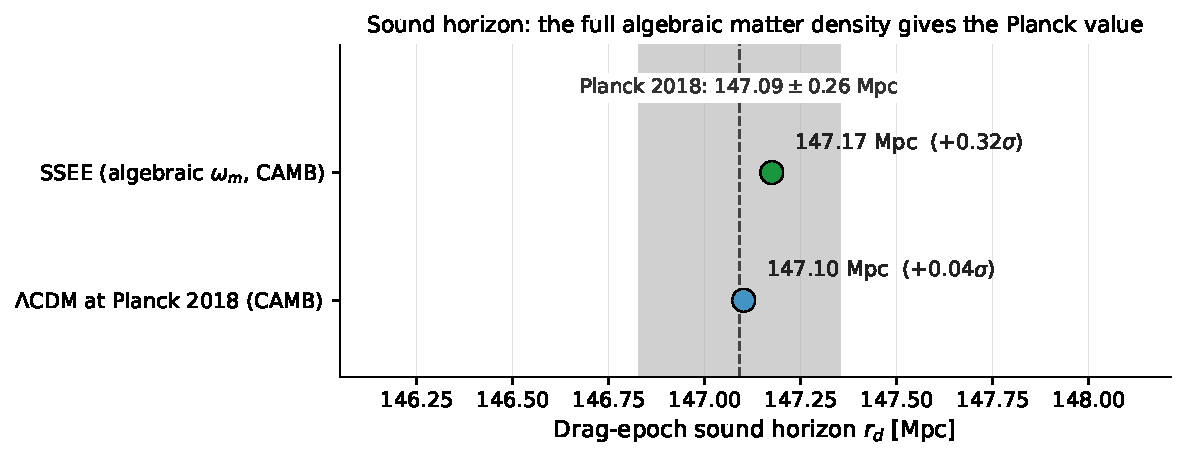
\includegraphics[width=0.82\textwidth]{fig_rd_dual.pdf}
  \caption{The physical sound horizon. Set by the full algebraic $\omega_m$
  (green, $147.17$~Mpc at $\Om^{\mathrm{cosm}}=0.308881$, $\omega_m$-direct), in
  agreement with Planck 2018 ($147.09\pm0.26$~Mpc, grey band) and the
  $\Lambda$CDM Eisenstein--Hu value (blue, $147.3$~Mpc); the BAO-distance run
  gives $148.2$~Mpc. This is the visual counterpart of the Boltzmann test above:
  the full matter density that restores the acoustic peaks also restores the BAO
  standard ruler. The $175.6$~Mpc scale (red) is the category error of using the
  cold sector $\Om^{\mathrm{dyn}}=0.160050$ as the background density.}
  \label{fig:rd_dual}
\end{figure}

\section{Bayesian validation: MCMC against DESI DR2}
\label{sec:mcmc}
The algebraic predictions of \S\ref{sec:core} are confronted with data in a
full Markov-chain Monte Carlo analysis. The dark-energy sector contributes no
sampled parameters---$w_0$, $w_a$ and the two-$\Om$ structure are fixed by
Eqs.~\eqref{eq:w0wa}--\eqref{eq:omcosm}---so the chain effectively samples
$H_0$ (and $\Omega_b h^2$) against the DESI DR2 BAO data with a CMB-derived
prior, using the affine-invariant ensemble sampler~\citep{emcee}. We ran $100$
walkers $\times\,25{,}000$ steps (seed $42$).

\paragraph{$H_0$ as one quantity in two stages.} We first anchor the
early-time geometry at the CMB-optimal value
\begin{equation}
  H_0^{\mathrm{anchor}} = H_0^{\rm alg} = 67.962~\kms ,
  \qquad
  \frac{H_0^{\rm alg}}{\kms} = 3(\varphi+\pi)^2 ,
  \label{eq:h0anchor}
\end{equation}
which (with $\omega_b,\omega_c$ fixed by SSEE algebra) is the $H_0$ that
minimises the Planck likelihood for the SSEE background; at this anchor the
sound horizon and acoustic scale are both well within tolerance,
$r_d = 147.17~\mathrm{Mpc}$ ($0.32\sigma$) and
$\theta_\ast = 0.59667^\circ$ ($1.00\sigma$). Letting the MCMC then correct
$H_0$ against the low-redshift BAO (corrected DESI~DR2 vector, block-diagonal
covariance with the official $r_{M,H}$ correlations) yields the posterior
\begin{equation}
  H_0^{\mathrm{post}} = 67.79 \pm 0.35~\kms ,
  \qquad
  \Omega_b h^2 = 0.02207 \pm 0.00045 ,
  \label{eq:h0post}
\end{equation}
with $r_d = 147.17~\mathrm{Mpc}$ ($0.32\sigma$, $\omega_m$-set, $H_0$-invariant)
at the posterior value. These are two stages of the same quantity---a CMB
anchor and a BAO-corrected posterior---and with the total matter density in the
background geometry they \emph{coincide}. (The earlier MIRA-anchored
$67.037/66.533$ stages, the $67.159$ posterior from the mislabelled DR1 vector,
and the $66.412$ obtained with the cold sector $0.160$ in the geometry, are all
superseded.)

\paragraph{Status of the algebraic anchor.} We are explicit about how a
dimensionful value is obtained from Eq.~\eqref{eq:h0anchor}, and about which
observable is the input. On its own, $3(\varphi+\pi)^2=67.962$ is a pure
number with no units; deriving the absolute scale of $H_0$ from first
principles is an open problem for every cosmological model, not only ours,
and we make no claim to have solved it. We therefore do not assert the pure
number as physical and then show that it explains the data. Instead we start
from the measured SH0ES \emph{local} rate,
$H_0^{\rm SH0ES}=73.04\pm1.04~\kms$~\citep{Riess2022}, and de-screen it with
the algebraically-derived (not fit) fraction $f_{\rm scr}=\alpha_K^{\rm eff}/(3\,\mathrm{MIRA})=(\pi-\varphi)/\Om^2=0.06725$
(Paper~9): $H_0^{\rm SH0ES}(1-f_{\rm scr})=68.13~\kms$, within $0.17\sigma$ of
the pure number $67.962$---the model-independent floor, using only the IR
screening term and no free parameter. Paper~10 sharpens this: with the
UV-completed fraction $f_{\rm scr}^{\rm UV}=\alpha_K^{\rm full}/(3\,\mathrm{MIRA})=0.069522$
(conditional on the derivation of $M^4=5\varphi^8\rho_{\rm crit}$ from UV--IR
$\varphi/\pi$ separability, Postulate~C.1), the identical inversion gives
$H_0^{\rm SH0ES}(1-f_{\rm scr}^{\rm UV})=73.04\times(1-0.069522)=67.9621~\kms$,
reproducing the anchor $3(\varphi+\pi)^2=67.9621$ to four decimals. We quote the
comparison at four decimals and not further because the input is quoted at two:
$H_0^{\rm SH0ES}=73.04$. We do not quote the reverse operation $3(\varphi+\pi)^2/(1-f_{\rm scr}^{\rm UV})$ as a prediction, because $3(\varphi+\pi)^2$
is a pure number and carries no units, so it cannot serve as the input of a
dimensionful cascade. The only directly measured expansion rate is the local
one, and Planck's is inferred within $\Lambda$CDM rather than measured; SH0ES
is therefore the input throughout. The leftover, $4\times10^{-6}~\kms$, lies below the resolution of
the datum it is compared against; whether a future, more precisely quoted local
measurement drives it down or opens it up is an empirical question, not one we
can settle here. We say ``to the quoted precision'' rather than ``exactly''
for that reason. We are deliberately precise about what is independent of what.
The de-screening is \emph{external}: it consumes only the measured SH0ES rate
and a screening fraction derived beforehand, with no SSEE value of $H_0$ as
input---but its two variants are one datum under two prescriptions, not two
independent measurements. The CMB/BAO chain, which never touches SH0ES, adopts
the anchor as its prior, so its posterior is a \emph{consistency} test rather
than a third confirmation: its content is that DESI DR2 does not pull the value
away ($\chi^2_{\rm BAO}\simeq10.3$ over 13 points, against $\simeq726$ for the
incorrect background geometry), leaving a residual displacement of
$0.50\sigma$. Replacing the anchor prior with a Planck one removes even that
dependence: the data then pull $H_0$ \emph{upward} from $67.36$ to
$67.53\pm0.35$, towards the anchor rather than away from it. That
pattern---one external datum and two independent-prior checks that decline to
move the value---is the anchor's physical content, not a claim that
$3(\varphi+\pi)^2$ literally equals a dimensionful rate. In Planck units
$H_0\sim10^{-61}$ and no such coincidence appears; the dimensional
origin---the bridge from the megaparsec scale to fundamental units---remains
open (\S\ref{sec:open}). The anchor is falsifiable on both fronts: a CMB/BAO
posterior displaced from it by more than $2\sigma$, or a SH0ES-derived local
rate that moves the unconditional IR floor outside $\sim1\sigma$, would
undermine it.

\paragraph{Anchor and posterior agree.} With the total gravitating matter
density $\Om^{\mathrm{cosm}}=0.308881$ in $E(z)$ and $r_d$, the BAO-corrected
posterior ($67.79$) and the CMB anchor ($67.962$) agree to $0.50\sigma$: DESI
DR2 is \emph{consistent with} the algebraic value rather than pulling against
it. All early-time observables are simultaneously healthy---$r_d=147.17$~Mpc
($0.32\sigma$) and, evaluating the acoustic scale at the posterior,
$100\,\theta_\ast=1.04089$ ($0.67\sigma$). The apparent $2.9\sigma$
``BAO--CMB split'' and the $13.9\sigma$ $\theta_\ast$ figure reported in earlier
drafts were the footprint of a single error---placing the cold dynamical sector
$\Om^{\mathrm{dyn}}=0.160050$ in the background geometry, where the total density
belongs. With that corrected, there is no split to report: the late-time BAO and
the early-time acoustic geometry point to the same $H_0$.

\paragraph{Model comparison against the natural competitors.} Because the
dark-energy sector carries no sampled parameters, the honest comparison is not
against $\Lambda$CDM alone but against the whole family a referee would reach
for. On the identical DESI~DR2 vector, the information criteria are:
\begin{table}[h]
\centering
\caption{Bayesian model comparison on DESI~DR2 ($100$ walkers $\times\,25{,}000$
steps). $\Delta$ values are relative to SSEE; positive favours SSEE.}
\label{tab:modelcomp}
\begin{tabular}{lccccc}
\toprule
Model & $k$ & $\ln P_{\rm MAP}$ & BIC & $\Delta$BIC & $\Delta$AIC \\
\midrule
SSEE          & 2 & $-5.47$ & $16.49$ & $0.00$  & $0.00$  \\
$\Lambda$CDM  & 3 & $-7.30$ & $22.92$ & $+6.43$ & $+5.65$ \\
CPL           & 5 & $-4.49$ & $22.85$ & $+6.35$ & $+4.04$ \\
\bottomrule
\end{tabular}
\end{table}
SSEE is favoured over both $\Lambda$CDM ($\Delta\mathrm{BIC}=6.43$) and CPL
($6.35$) by parsimony, with $\Delta\mathrm{DIC}=-5.66$ and a Savage--Dickey factor
$\ln B=2.90$ (substantial on the Jeffreys scale); a leave-one-out
cross-validation at $z\ge1$ ranks SSEE ahead of both ($\chi^2_r=0.21$ versus
$0.71$ for $\Lambda$CDM and $39.6$ for CPL). The preference is driven by fewer
parameters at equal fit, not by a superior $\chi^2$: the competitor that
\emph{can} bend to the data (CPL, $k=5$) is penalised for the freedom SSEE does
not use.

\begin{figure}[t]
  \centering
  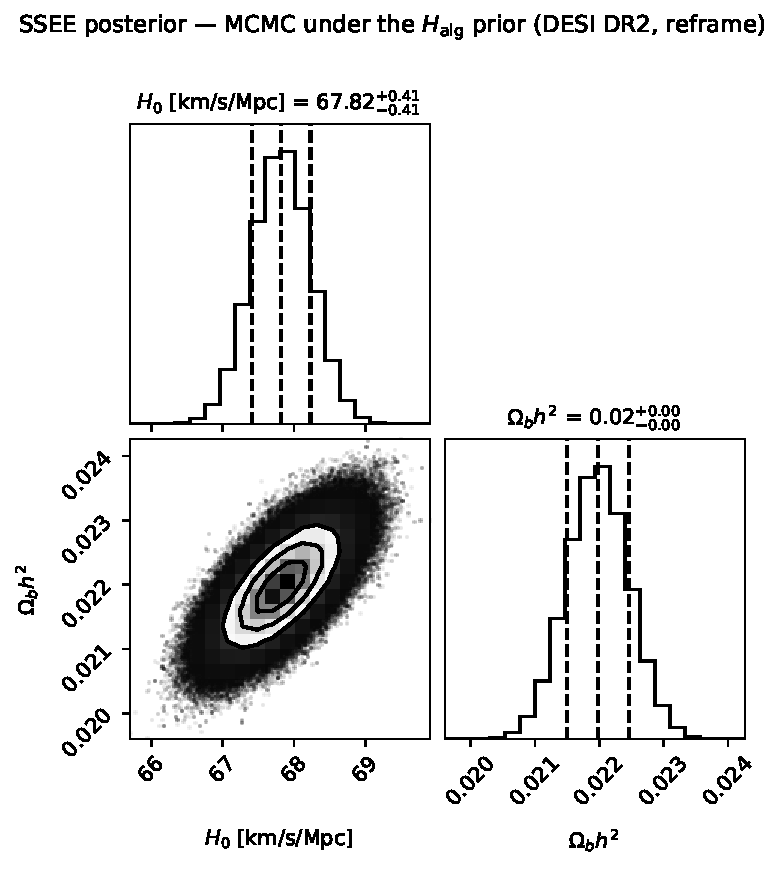
\includegraphics[width=0.62\textwidth]{fig_corner_ssee_halg_prior.pdf}
  \caption{Marginalised posterior from the MCMC analysis ($100$ walkers
  $\times\,25{,}000$ steps). With the entire dark-energy sector fixed by
  $\varphi$ and $\pi$, the chain samples only $H_0$ and $\Omega_b h^2$ against
  DESI DR2 BAO with the $\omega_m$-direct CMB anchor as prior. The posterior is
  $H_0=67.79\pm0.35~\kms$ and $\Omega_b h^2 = 0.02207\pm0.00045$
  (Eq.~\ref{eq:h0post}), agreeing with the anchor to $0.50\sigma$. Dashed lines
  mark the anchor inputs $(H_0=67.962~\kms,\ \Omega_b h^2 = 0.02218)$; the
  $16/50/84\%$ quantiles are indicated.}
  \label{fig:corner}
\end{figure}

\section{The CMB and the effective field theory}
\label{sec:eft}

The equation-of-state construction of \S\ref{sec:core} fixes the
late-time expansion history. To test the framework against the cosmic
microwave background and large-scale structure we must specify its behaviour
at the level of linear perturbations. We do so through an effective field
theory (EFT) of dark energy whose functions are again fixed by $\varphi$ and
$\pi$, with no perturbation-level parameters introduced beyond those already
present in the background.

\subsection{The effective field theory of the dark sector}
\label{sec:eft-functions}
In the EFT-of-dark-energy language \citep{Cheung2008,Gubitosi2013,Bellini2014} the linear
dynamics of a single scalar degree of freedom are controlled by four
functions $\alpha_{\rm K}$ (kineticity), $\alpha_{\rm B}$ (braiding),
$\alpha_{\rm M}$ (Planck-mass run) and $\alpha_{\rm T}$ (tensor speed excess).
SSEE fixes them algebraically:
\begin{equation}
  \label{eq:eft-alphas}
  \alpha_{\rm T}=\alpha_{\rm M}=\alpha_{\rm B}=0,
  \qquad
  \alpha_{\rm K}(0)=3\,\Omega_{\rm DE}\,\Om^{\mathrm{dyn}}=0.403302 ,
  \qquad
  \Omega_{\rm DE}=\mathrm{AURA}/\Omega=1-\Om^{\mathrm{dyn}}=0.839950 ,
\end{equation}
so that gravitational waves propagate at the speed of light
($\alpha_{\rm T}=0$, consistent with GW170817~\citep{GW170817}) and the only non-trivial
function is the kineticity, set by the same dynamical matter fraction
$\Om^{\mathrm{dyn}}=0.160050$ that appears in the background. We cross-checked
$\alpha_{\rm K}(0)$ with the Bellini--Sawicki implementation in \texttt{hi\_class}
\citep{Bellini2015} and recovered $0.4033$ to within $0.005\%$. The associated conformal coupling
of the scalar to matter is
\begin{equation}
  \label{eq:betac}
  \beta_c=-\mathrm{AURA}=-3.997847 ,
\end{equation}
extracted from the requirement that the field's present energy fraction equal
$\Omega_{\rm DE}$. \textbf{Withdrawn (2026-09-07).} Earlier versions reported
$\beta_c\simeq-3.98991$, agreeing with $-\mathrm{AURA}$ at the $0.2\%$ level,
and offered that numerical value as the robust statement. Both claims are
withdrawn. The agreement was an artefact of a normalisation bug: the shooting
calibrated $\Omega_\phi(a{=}1)$ to the saturation $0.839950$ instead of the
density $0.691119$; corrected, the coupled background returns
$\beta_c=-2.194210$, at $45\%$ of $\mathrm{AURA}$. More decisively, Paper~7
has since withdrawn the conformal coupling altogether along with the potential
--- the operative Lagrangian $K(X)=c_1X+c_2X^2$ contains neither --- so there
is no $\beta_c$ left to identify. No published number was a function of it.
What remains open is a different question, tracked as OP-24: no background
reproduces $w_a=-0.669975$, and the difficulty lies in the \emph{form} of the
potential.

\subsection{Inflationary sector: $\alpha$-attractor}
\label{sec:inflation}
The primordial perturbations are described by an $\alpha$-attractor
\citep{Kallosh2013} with curvature
\begin{equation}
  \label{eq:alpha-attractor}
  \alpha=\frac{\varphi^4}{3}=2.284701 .
\end{equation}
For the attractor universality class, $n_s=1-2/N_\ast$ and
$r=12\alpha/N_\ast^2$. We take the number of $e$-folds to be
$N_\ast=2\varphi^7=58.068884$. The coefficient $2$ is not a free choice. Within
the observationally allowed window $[50,60]$ the products $m\varphi^n$ with
small integer $m$ are $2\varphi^7$, $3\varphi^6$, $5\varphi^5$ and $8\varphi^4$;
of these, $m=2$ is the only one for which the spectral index comes out as a pure
power of $\varphi$, precisely because that $2$ cancels against the $2$ in
$n_s=1-2/N_\ast$ (the others give $1-\varphi^{-6.84}$, $1-\varphi^{-6.90}$ and
$1-\varphi^{-6.88}$). The same coefficient simultaneously renders $r$ a pure
power. $N_\ast=2\varphi^7$ is therefore the unique member of that family for
which \emph{both} observables reduce to pure powers of $\varphi$, and the two
resulting identities are exact:
\begin{equation}
  \label{eq:ns-r}
  n_s = 1-\varphi^{-7}=0.965558 ,
  \qquad
  r   = \varphi^{-10}=8.130619\times10^{-3} .
\end{equation}
The spectral index sits squarely on the Planck~2018 measurement
($n_s=0.9649\pm0.0042$;~\citealp{Planck2018}); the tensor-to-scalar ratio
$r=\varphi^{-10}$ is a
pre-committed, falsifiable prediction (\S\ref{sec:falsifiability}) well below
the current bound $r<0.036$ and within reach of LiteBIRD and CMB-S4. We note
that, within the framework, $n_s$ and $r$ are postulated of this form and
$\alpha=\varphi^4/3$ then follows as an exact algebraic consequence; we do not
claim an independent derivation of the exponent~$7$ from the potential
(see~\S\ref{sec:open}).

\subsection{Confrontation with Planck PR4}
\label{sec:cmb-confront}
With the background of \S\ref{sec:core} and the EFT functions of
Eq.~\eqref{eq:eft-alphas}, we computed the CMB angular power spectra with the
\texttt{CLASS} Boltzmann code~\citep{Lesgourgues2011} and compared against
Planck PR4~\citep{PlanckPR4} (TT, TE, EE and lensing).
Table~\ref{tab:cmb} reports the reduced $\chi^2$.

\begin{table}[t]
  \centering
  \begin{tabular}{lccc}
    \toprule
    Spectrum & SSEE $\chi^2_r$ & $\Lambda$CDM $\chi^2_r$ & $N$ \\
    \midrule
    TT          & 1.042 & 1.043 & 1971 \\
    TE          & 1.040 & 1.040 & 1967 \\
    EE          & 1.040 & 1.039 & 1967 \\
    $\phi\phi$ (lensing) & 0.720 & 0.757 & 9 \\
    \bottomrule
  \end{tabular}
  \caption{CMB confrontation against Planck PR4. SSEE reproduces the acoustic
  spectra at a quality indistinguishable from $\Lambda$CDM, with acoustic peaks
  at $\ell=220,\,535,\,810$. The combined $\Delta\mathrm{BIC}
  (\text{SSEE}-\Lambda\text{CDM})=-35.0$ over $N=5914$ data points (diagonal,
  $\omega_m$-direct) reflects the two-parameter economy of the background.}
  \label{tab:cmb}
\end{table}

\paragraph{Which likelihood the model comparison rests on.} We are explicit
about this because the two numbers differ and only one of them is a model
comparison. The $\chi^2_r$ of Table~\ref{tab:cmb} and the associated
$\Delta\mathrm{BIC}=-35.0$ use a \emph{diagonal} covariance. That is adequate
for displaying spectral agreement, but not for selecting between models:
neglecting the Planck bandpower correlations overstates the number of
independent data points, and since the BIC penalty enters as $k\ln N$, it
inflates precisely the term that rewards the smaller $k$. We therefore also
evaluate the compressed Planck likelihood \texttt{plik\_lite}
(TT+TE+EE, $613$ bandpowers, nuisance parameters marginalised by the Planck
Collaboration) together with the low-$\ell$ TT and EE likelihoods, for $N=669$
data points, which gives $\chi^2_{\rm SSEE}=1003.586$ against
$\chi^2_{\Lambda\rm CDM}=1003.769$ with $\{A_s,\tau\}$ minimized in both---an
equal fit ($\Delta\chi^2=-0.183$, statistically zero) for four fewer free
parameters---and
\begin{equation}
  \label{eq:dbic-cmb}
  \Delta\mathrm{BIC}(\text{SSEE}-\Lambda\text{CDM}) = -26.21 \qquad
  (\texttt{plik\_lite}, k=2 \text{ vs } 6) .
\end{equation}
This is the number the model comparison rests on; the diagonal $-35.0$ is
retained for continuity with Paper~3 and should be read as illustrative. One
residual dependence would remain---\texttt{plik\_lite} marginalises its nuisance
parameters within a $\Lambda$CDM analysis---so we also ran the \emph{full}
\texttt{plik} likelihood (TTTEEE $+$ lowl TT $+$ lowl EE $+$ lensing,
$N=2354$) with the ${\sim}20$ nuisance parameters sampled explicitly. That chain
has converged (Gelman--Rubin $R-1=0.017$) and it strengthens the result rather
than softening it:
\begin{equation}
  \label{eq:dbic-full}
  \chi^2_{\rm SSEE}=2770.44 , \quad \chi^2_{\Lambda\rm CDM}=2772.92 , \quad
  \Delta\mathrm{BIC}=-25.77 \qquad (\texttt{plik full}, k=3 \text{ vs } 6) .
\end{equation}
With the nuisance parameters free, SSEE attains a \emph{better} fit than
$\Lambda$CDM---by $\Delta\chi^2=-2.47$---using three fewer free parameters,
where under \texttt{plik\_lite} it paid $+1.65$. Sampling $H_0$ freely in the
same chain returns $H_0=67.88\pm0.10~\kms$, within $0.81\sigma$ of the algebraic
anchor $3(\varphi+\pi)^2=67.962$: the chain \emph{recovers} the anchor rather
than assuming it, and its uncertainty is $5.3\times$ tighter than the
$\Lambda$CDM posterior on the same data, as the parameter economy predicts.

\begin{figure}[t]
  \centering
  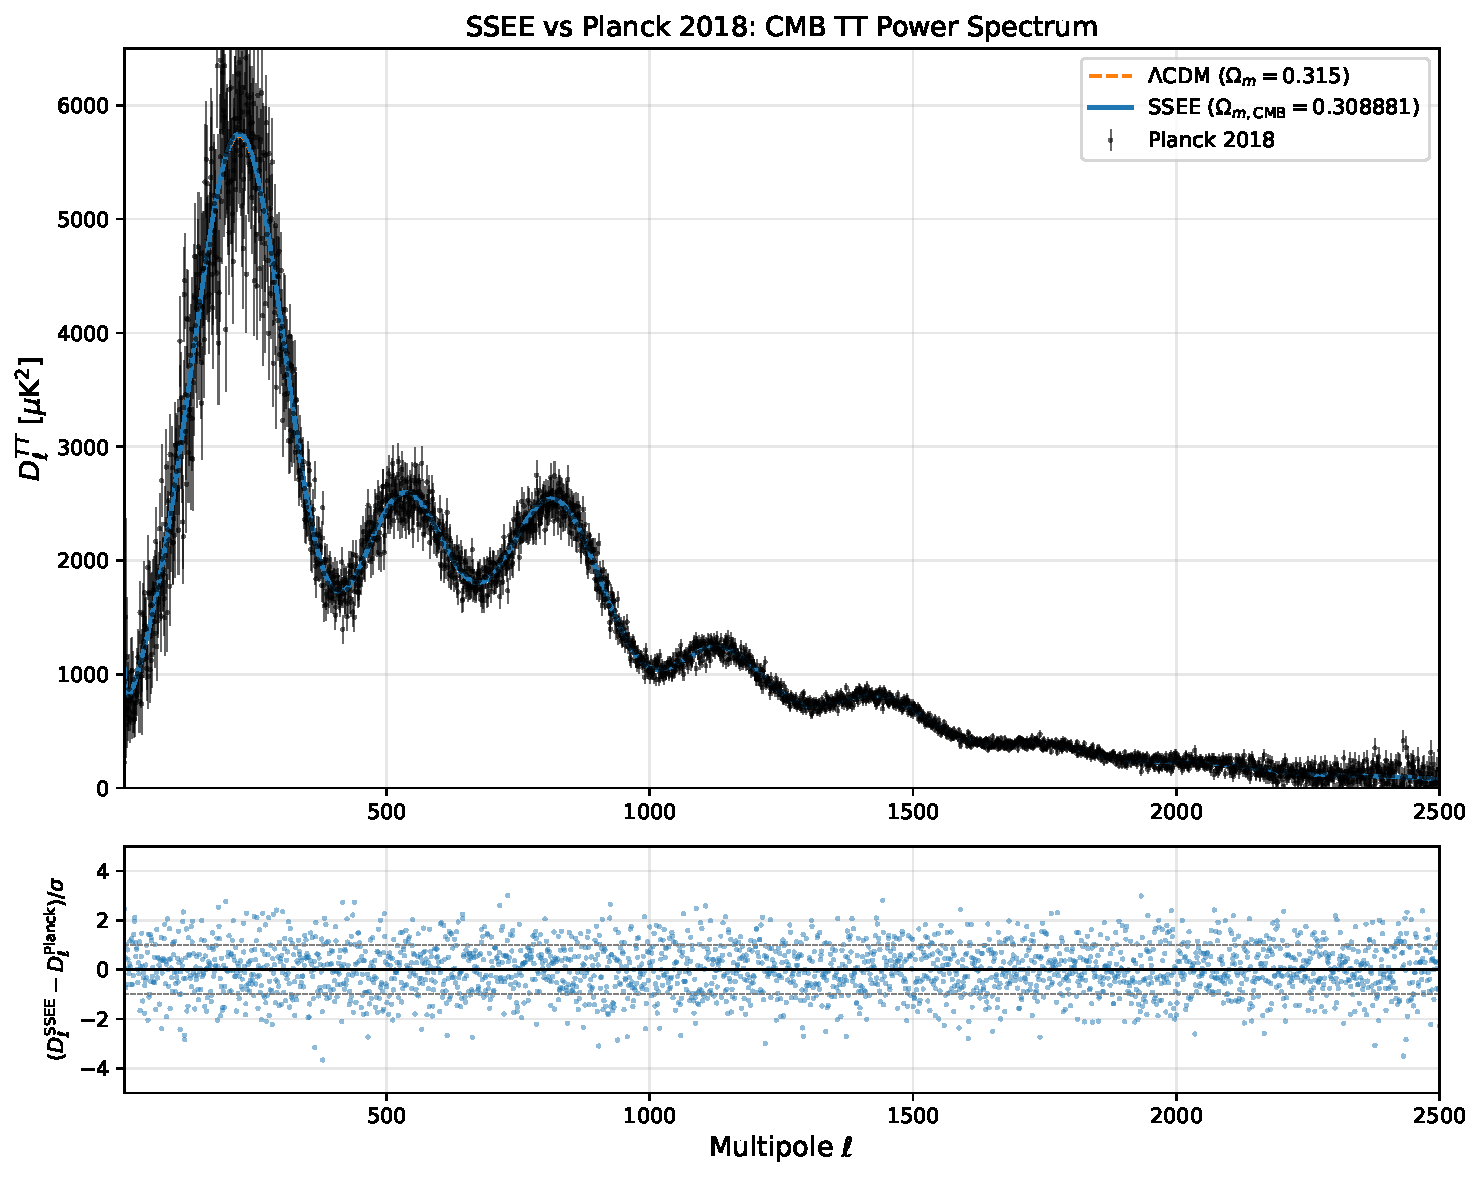
\includegraphics[width=0.82\textwidth]{fig_cmb_spectrum.pdf}
  \caption{CMB temperature angular power spectrum computed with \texttt{CLASS}
  for the SSEE background and EFT functions (Eq.~\ref{eq:eft-alphas}), compared
  against Planck PR4. With the dark-energy sector fixed by $\varphi$ and $\pi$,
  SSEE reproduces the acoustic peaks at $\ell=220,\,535,\,810$ at a quality
  indistinguishable from $\Lambda$CDM (Table~\ref{tab:cmb}). The two-$\Om$
  structure is essential: replacing $\Om^{\mathrm{cosm}}=0.308881$ with the bare
  $\Om^{\mathrm{dyn}}=0.160050$ shifts every peak by ${\sim}10\%$.}
  \label{fig:cmb}
\end{figure}

\paragraph{The CMB density is physically required, not cosmetic.}
The two-$\Om$ structure
of \S\ref{sec:two-omega} is decisively tested by the CMB. Running the Boltzmann
solver at the cosmological matter fraction $\Om^{\mathrm{cosm}}\approx0.31$ (a
CLASS validation at $0.320$; the $\omega_m$-direct canonical $0.308881$ lies
within $3.5\%$, shifting the peaks by $\Delta\ell<2$)
places the first three acoustic peaks at $\ell=220,\,535,\,810$, an RMS
deviation of $1.4\%$ from $\Lambda$CDM. Running it instead with the bare
dynamical fraction $\Om^{\mathrm{dyn}}=0.160050$ shifts all
three peaks by ${\sim}10\%$ ($\ell=240,\,597,\,922$) and raises the RMS to
$31.5\%$---a factor of ${\sim}22$ worse. The sound horizon at recombination
therefore \emph{demands} $\Om^{\mathrm{cosm}}\approx0.31$: the CMB matter density
is not a fit applied
to the data but a structural feature without which the model fails the CMB
outright. Its numerical value follows from the $\omega_m$-direct identity
($\omega_c=\mathrm{KAL_0}\,\omega_b\,n_s$, fixed by $\varphi,\pi$; \S\ref{sec:open}).

\section{Structure growth: an honest tension}
\label{sec:growth}

The same linear EFT predicts the growth of structure, and here we report the
situation honestly: a genuine challenge in the minimal (single-sector)
treatment, resolved only by an extension sector that we deliberately keep
outside the core register. With the Poisson source evaluated at the
CMB-calibrated density $\Om^{\mathrm{cosm}}=0.308881$ ($\omega_m$-direct, the
structure that the Boltzmann test of \S\ref{sec:eft} shows is
physically required), the growth factor is essentially that of $\Lambda$CDM,
$G\equiv D_1^{\rm SSEE}/D_1^{\Lambda\rm CDM}=1.0032\pm0.005$, and the
single-sector amplitude ceiling (CLASS forward) is
\begin{equation}
  \label{eq:s8}
% ACTUALIZADO 2026-09-08: era sigma_8=0.8335 / S_8=0.846 (tensiones 1.1/3.5/3.9
% sigma). Ese numero salia de una corrida CLASS sin .ini, fuera del repo y SIN
% neutrinos masivos; el fondo canonico si los lleva (Sum m_nu = 0.06849 eV) y sin
% ellos sobra un 2.3% de grumo. Re-corrido con config/class/techo_ssee_canonico.ini;
% control con criterio previo (baseline Planck debe dar 0.8111+/-0.006) da 0.810851.
% Log: results/logs/p5_techo_sigma8_As_fijo.json
  \sigma_8=0.8149\pm0.006 , \qquad S_8=0.827
\end{equation}
when the primordial amplitude $A_s$ is held at the Planck-preferred value.
That configuration was previously reported as a $3.5\sigma$ tension with
KiDS-1000~\citep{KiDS2021,DESY32022}, and a two-sector $\varphi$-DM extension
was proposed to resolve it. \textbf{Both the tension and the extension are
withdrawn here}, for two independent reasons.

First, fixing $A_s$ to Planck is not a neutral choice: $A_s$ is one of the two
free parameters this model retains at CMB level, so a number obtained that way
reports the Planck--shear disagreement rather than a property of the model.
That disagreement is real and is not resolved here --- asking this model's own
CMB fit to set $A_s$, rather than borrowing Planck's, still leaves
$3.4\sigma$ against the shear determination. Second, the target itself was model-conditioned: the published $S_8$
is a compressed statistic whose data-reduction pipeline assumes a $\Lambda$CDM
background, so fitting to it compares a non-$\Lambda$CDM model against a
partly-$\Lambda$CDM number.

Measured instead against the 225 \emph{raw} KiDS-1000 $\xi_\pm$ data points,
with the background fixed entirely by the algebra, a \emph{single}
unpartitioned matter sector $\Omega_m=0.308881$, and only $A_s$ and the eight
official nuisance parameters free, a converged MCMC ($R-1=0.019$,
$4.2\times10^4$ effective samples) gives
\begin{equation}
  \sigma_8 = 0.7446\pm0.0189, \qquad S_8 = 0.7555\pm0.0192,
\end{equation}
i.e.\ $0.11\sigma$ from the KiDS-1000 value $0.759\pm0.024$ --- and, in the like-for-like comparison, $\Delta S_8=0.0016$ from the $\Lambda$CDM control run through the same pipeline ($0.7571\pm0.0194$), with
$\chi^2_{\rm min}=265.4$ over $216$ degrees of freedom. \textbf{There is no
$S_8$ tension to resolve, and therefore nothing for a second sector to do.}

\paragraph{The same test against KiDS-Legacy.}
The measurement above uses KiDS-1000.  Repeating it against the KiDS-Legacy
release---357 raw $\xi_\pm$ points, Wright et al.\ (2025) (arXiv:2503.19441),
published sixteen months before the present analysis, over which we claim no
temporal priority---closes the sector.  With the same algebraic background and
$A_s$ free, the shear asks for $\log(10^{10}A_s)=3.0255\pm0.0396$, against the
$3.04483$ that the CMB fixes \emph{under that same background}: a distance of
$0.49\sigma$.  The control with the Planck background held equally rigid gives
$1.01\sigma$.  Fixing $A_s$ to the CMB value therefore costs nothing:
\begin{equation}
  \chi^2 = 417.97 \ \ (\text{8 free, all nuisance, \emph{none} cosmological})
  \quad\text{vs.}\quad
  418.34 \ \ (A_s \text{ free}),
\end{equation}
over the same 357 points, giving $\Delta\mathrm{BIC}=+6.24$ in favour of the
fixed-amplitude model, and $+6.86$ against the $\Lambda$CDM-background control
($418.95$).  With no free cosmological parameter left, $S_8=0.8273$ is a
prediction rather than a fit, against $0.8265\pm0.0176$ measured---$0.05\sigma$.

Two cautions belong with this result.  The three $\chi^2$ values span $1.0$
over 357 points: \textbf{the shear does not discriminate between these
models}, and we do not claim that it does.  What separates them is the number
of parameters each had to spend and whether $A_s$ stays consistent between the
CMB and the growth epoch.  And the earlier KiDS-1000 release asked for
$\log(10^{10}A_s)=2.863\pm0.051$, $3.5\sigma$ from the same target; the two
releases differ from each other by $2.5\sigma$.  What changed is the data---the
$n(z)$ calibration, by the collaboration's own Appendix~I---not the model.  A
future release returning to the lower amplitude would reopen the sector.

The $\varphi$-DM component and its particle are retracted independently of
this: the subtraction that defined the second sector's density,
$\Omega_{\varphi\rm DM}=\Omega_{m,\rm CMB}-\Omega_{m,\rm dyn}$, took a measured
density minus $1+w_0$ --- a number from the equation of state, not a density.
The subtraction is arithmetically well formed and physically empty, so the
particle had nothing to be made of.

\begin{figure}[ht]
  \centering
  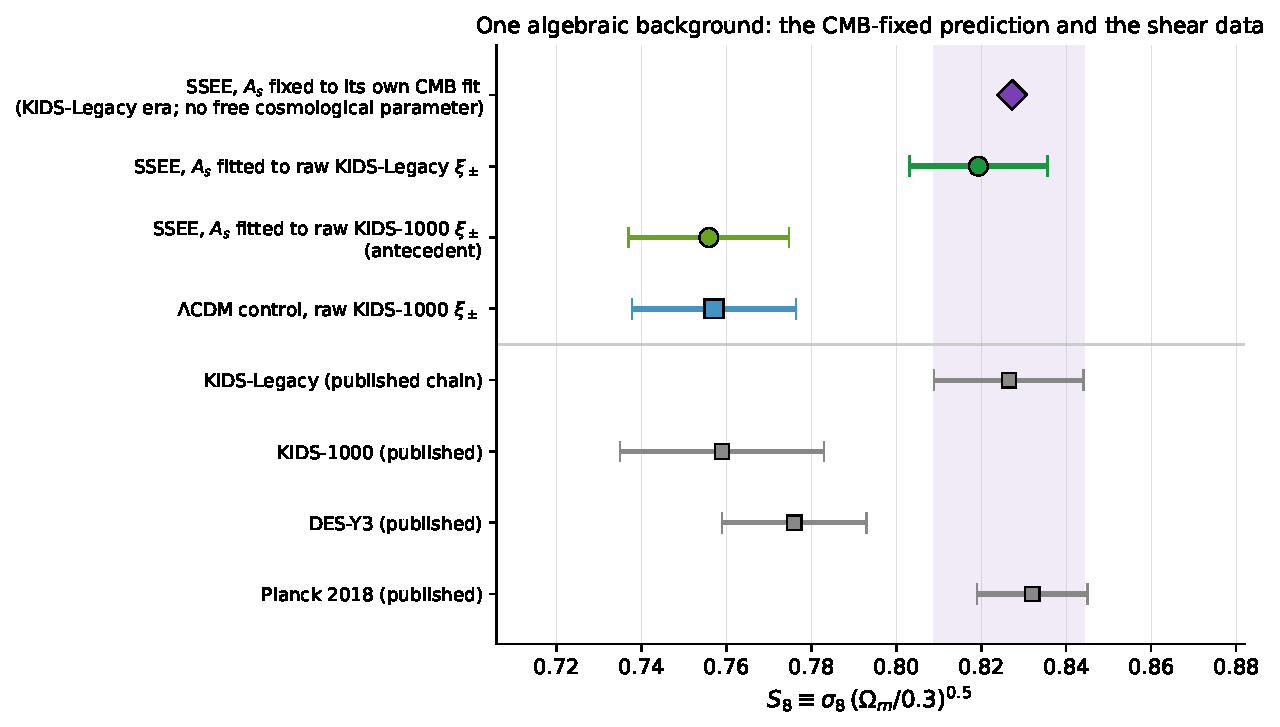
\includegraphics[width=0.9\textwidth]{fig_s8_resolution.pdf}
  \caption{$S_8$ with the primordial amplitude fixed versus fitted. The single-sector ceiling (red, $S_8=0.827\pm0.006$)
  carries the $3.5\sigma$ tension with KiDS-1000 reported in
  Eq.~\eqref{eq:s8}; fitting $A_s$ to raw $\xi_\pm$ data (green,
  $S_8=0.7555\pm0.0192$) lands $0.11\sigma$ from KiDS-1000 (green band); the $\Lambda$CDM control on the same raw data lands at $0.7571\pm0.0194$. The
  retracted two-sector curve is no longer shown, and the
  free-streaming scale it used is withdrawn with the
  particle. Grey
  points: Planck 2018, KiDS-1000 and DES-Y3 with $1\sigma$ errors.}
  \label{fig:s8_resolution}
\end{figure}

\paragraph{The honest statement.} The single-sector core of SSEE does not
resolve the $S_8$ tension---it inherits it at the $\Lambda$CDM level. The
retracted extension appeared to resolve it, but the UV
origin of the algebraic multiplier that fixes $m_\varphi$ remains underived
(OP-9, now closed by dissolution with the retracted sector), so the extension stayed outside the core predictive register, and a
full non-linear treatment requires $N$-body simulations that lie beyond the
scope of this work. We report the core-level tension as an open challenge
(\S\ref{sec:open}) and the withdrawn extension as a cautionary record,
not a claimed first-principles victory.

\section{Falsifiability and the prediction register}
\label{sec:falsifiability}

The defining property of a parameter-frugal framework is that, once the
algebraic invariants are fixed, the numbers it predicts are not free to move.
A fit can always be improved by adding a parameter; SSEE has none to add. We
therefore commit, in advance, to a register of quantitative predictions, each
attached to the observation that will confirm or refute it. We separate the
register into two tiers: \emph{core} predictions that follow directly from the
dimensionless invariants $\varphi$ and $\pi$, and \emph{extension} predictions
that depend on the phenomenological $\varphi$-dark-matter sector and are
therefore conditional on assumptions still under investigation
(\S\ref{sec:open}).

\subsection{Master register: one line per observable}
\label{sec:master-register}

Before the two tiers in detail, Table~\ref{tab:master} gives the entire suite
on a single page: every confronted observable, the sector it belongs to, the
paper that derives it, its algebraic value, and its epistemic status
(postdiction / retrodiction / prediction / measured input). The horizontal rule
separates the \emph{core} tier---fixed by $\varphi$ and $\pi$ alone---from the
\emph{extension} tier, which depends on the phenomenological $\varphi$-dark-matter
sector. This is the navigation map for the whole programme; each row is expanded
in the paper named in its last-but-one column and in the Predictive Register of
Paper~1.

\begin{table}[h]
\centering
\small
\resizebox{\textwidth}{!}{%
\begin{tabular}{@{}lllll@{}}
\toprule
Observable & Sector & Value & Paper & Status \\
\midrule
\multicolumn{5}{l}{\textit{Core tier --- clean from $\varphi,\pi$ (no fitted coefficient)}} \\
$w_0=-T_r/M_v$                & Background (DE)   & $-0.839950$                         & P1,2,4 & Postdiction \\
$w_a=-P_{\rm sc}/I_g$ & Background (DE)   & $-0.669975$                      & P1,2,4 & Postdiction \\
$(w_0,w_a)$ vs DESI DR3       & Background (DE)   & same fixed point                & P1,2   & \textbf{Prediction (pre-reg.)} \\
$H_0/\kms=3(\varphi+\pi)^2$   & Background (DE)   & $67.962\,\kms$                   & P1,2,9 & Global anchor (Post.~D) \\
$\omega_c=\mathrm{KAL}_0\,\omega_b\,n_s$ & CMB      & $0.119514$                       & P1,3   & Retrodiction \\
$\Om^{\rm cosm}=\omega_m/h^2$ & CMB               & $0.308881$                       & P1,3   & Retrodiction \\
$n_s=1-\varphi^{-7}$          & Inflation / CMB   & $0.965558$                       & P1,3   & Retrodiction \\
$r=\varphi^{-10}$             & Inflation         & $8.1\times10^{-3}$              & P1     & \textbf{Prediction} \\
$\alpha_T=\alpha_M=\alpha_B$  & EFT               & $0$ (exact)                     & P7     & Retrodiction \\
$\alpha_K^{\rm field}$ (bare, pre-integration) & EFT & $0.073$                        & P7     & Internal check \\
$\beta_c=-\mathrm{AURA}$      & EFT               & $-3.997847$                        & P7     & Retrodiction \\
$\gamma_{\rm IS}$ (Israel--Stewart) & Growth      & $0.550$                         & P5     & Retrodiction \\
$f\sigma_8$ (single-sector)   & Growth            & $0.70\sigma$ (6 RSD)            & P5     & Retrodiction \\
\midrule
\multicolumn{5}{l}{\textit{Extension tier --- depends on the $\varphi$-dark-matter sector}} \\
$S_8$ (KiDS-Legacy, $A_s$ fixed by CMB) & growth & $0.8273$ predicted vs.\ $0.8265\pm0.0176$ ($0.05\sigma$) & P6 & \textbf{Prediction} \\
$S_8$ (KiDS-1000, $A_s$ free) & growth  & $0.7555\pm0.0192$ ($\Lambda$CDM ctrl $0.7571$) & P6 & Retrodiction \\
$M=(5\varphi^8\rho_{\rm crit})^{1/4}$ & UV compl.  & $9.68\,$meV                    & P10    & Derived (UV) \\
Lensing (canonical EFT)       & Strong gravity    & GR$+$DM (uncond.)              & P8     & Retrodiction \\
\midrule
\multicolumn{5}{l}{\textit{Measured input (not derived)}} \\
$A_s,\ \tau$                  & CMB amplitude     & sampled ($k=2$)                & P1,3   & Measured \\
$\rho_{\rm vac}$ (abs.\ scale) & Vacuum            & single measured input          & P1,10  & Measured \\
\bottomrule
\end{tabular}%
}
\caption{Suite-wide master register: one row per observable across the ten-paper
programme. ``Postdiction'': algebraic result fixed by the closed dictionary, then
compared to already-public data (no claim of temporal priority). ``Retrodiction'':
derived independently, then compared to an existing measurement. ``Prediction'':
fixed now, tested against not-yet-released data. ``Measured'': an input, not a
derivation. ``Internal check'': a same-paper consistency quantity, not itself
tested against external data. No optimisation over the algebraic formula space
was performed. The bare-field $\alpha_K^{\rm field}=0.072567$ (Paper~7) is the
pre-integration kinetic contribution, distinct from the background-integrated
$\alpha_K(0)=0.403302$ used and cross-checked against \texttt{hi\_class} in
\S\ref{sec:eft-functions}: both are Paper~7 quantities at different stages of
the same calculation, not competing values for the same object. The detailed
per-sector registers follow below and in the Predictive Register of Paper~1.}
\label{tab:master}
\end{table}

\subsection{Core predictions (clean from $\varphi,\pi$)}

These quantities carry no fitted coefficient. They are bare ratios of the
golden mean and $\pi$, and they cannot be adjusted to accommodate data.

\begin{table}[h]
\centering
\begin{tabular}{@{}llll@{}}
\toprule
Observable & SSEE value & Algebraic form & Falsifying probe \\
\midrule
$w_0$            & $-0.839950$              & $-T_r/M_v$            & DESI Y3 / Euclid BAO+SNe \\
$w_a$            & $-0.669975$              & $-P_{\rm sc}/I_g$ & DESI Y3 / Euclid BAO+SNe \\
$n_s$            & $0.965558$               & $1-\varphi^{-7}$      & Planck / CMB-S4 \\
$r$              & $8.1306\times10^{-3}$     & $\varphi^{-10}$       & LiteBIRD / CMB-S4 \\
$\alpha_K(0)$    & $0.403302$               & $3\,\Omega_{\rm DE}\,\Om^{\mathrm{dyn}}$ & DESI / Euclid growth \\
$\alpha_T,\alpha_M,\alpha_B$ & $0$        & exactly zero          & GW standard sirens, ISW \\
\bottomrule
\end{tabular}
\caption{Core prediction register. Each value is fixed by $\varphi$ and $\pi$
alone, with no free parameter available to absorb a discrepancy. The tensor
ratio $r=\varphi^{-10}$ sits an order of magnitude below the current bound
$r<0.036$ and is the cleanest single falsification target: a detection above
$\sim10^{-2}$, or a robust upper bound below $\sim8\times10^{-3}$, refutes the
inflationary sector.}
\label{tab:predictions-core}
\end{table}

The tensor-to-scalar ratio deserves emphasis. Because $n_s=1-\varphi^{-7}$ and
$r=\varphi^{-10}$ are postulated to be of this form, the consistency relation of
the underlying $\alpha$-attractor closes algebraically: with $N_*=2\varphi^7$
and $\alpha=\varphi^4/3$ one obtains
$r=12\alpha/N_*^2=12(\varphi^4/3)/(2\varphi^7)^2=\varphi^{-10}$ identically. The
prediction is thus internally locked rather than independently adjustable. Its
value, $r\simeq8.1\times10^{-3}$, lies squarely within the reach of LiteBIRD and
CMB-S4, which target $\sigma(r)\sim10^{-3}$. SSEE will be decisively tested by
the next generation of $B$-mode experiments.

\paragraph{A pre-registered DESI DR3 test.} The equation-of-state point is
fixed forever at $(-0.840,-0.670)$; each DESI release is therefore a fresh
blind test of the \emph{same} target. The trajectory to date: against the legacy DR1 posterior the
point sat at ${\sim}0.05\sigma$; against DR2,
whose uncertainties are ${\sim}40\%$ tighter, it sits at $0.24\sigma$
(Pantheon+; \S\ref{sec:desi-agreement})---the contour shrank and the fixed
point stayed inside the $68\%$ region, which a fitted model can always do but
a rigid one need not. We pre-commit, in advance of the DR3 release (expected
2027), to the following quantitative expectations for
DESI DR3, whose uncertainties are forecast to improve by ${\sim}1.5\times$:
if the DR2 central values persist, the point will sit at ${\sim}0.5\sigma$ of
the DR3$+$CMB$+$Pantheon+-class posterior (still inside $1\sigma$), while the
Union3/DESY5-class combinations would sharpen to ${\sim}2.2$--$2.7\sigma$
---DR3 will therefore \emph{discriminate among the supernova compilations}
whose spread already dominates the range quoted in \S\ref{sec:desi-agreement}.
The falsification line is pre-registered \emph{now}, before the DR3 release, and
fixed to a specific supernova compilation so that no post-hoc choice of sample can
rescue the model: a joint exclusion of $(-0.840,-0.670)$ at ${>}3\sigma$ in the
DR3 $w_0$--$w_a$ plane for the DR3\,$+$\,CMB\,$+$\,\emph{Pantheon+} combination
---the same Pantheon+ compilation used for the headline agreement throughout this
work---refutes the algebraic background. We will additionally report the
Union3- and DESY5-class combinations for completeness, but the pre-committed
falsifier is the Pantheon+ line named here. No parameter exists with which
to absorb such an outcome.

The vanishing of the EFT slip functions $\alpha_T=\alpha_M=\alpha_B=0$ is
equally sharp: SSEE predicts a gravitational-wave speed identical to light
($c_T=c$) to all orders in the dark sector, no running of the effective Planck
mass, and no braiding. Any measured departure---an anomalous standard-siren
distance, a time-varying $G_{\rm eff}$, or a non-zero braiding signature in the
ISW--galaxy cross-correlation---falsifies the canonical EFT presented in
\S\ref{sec:eft}.

\section{Honest accounting and outstanding challenges}
\label{sec:open}

A framework is only as credible as its honesty about what it does not yet
explain. We therefore state plainly the inputs the model still requires, the
exact parameter count, and the principal open problems---not as caveats buried
in a footnote, but as the research agenda that the present work both motivates
and constrains.

\subsection{What is measured, not derived: the vacuum scale}

SSEE does not predict the absolute energy density of the dark sector. The
overall scale of the vacuum, $\rho_\Lambda\simeq6\times10^{-10}~\mathrm{J\,
m^{-3}}$, enters as a single measured input, which we label \emph{Postulate~D}.
What the algebra fixes is the \emph{shape} of the dark-energy sector---its
equation-of-state ratios $w_0,w_a$, the two-$\Omega$ structure, and the EFT
function profile---not its amplitude. We make no claim to have solved the
cosmological-constant problem; we have moved its free numbers from six tuned
cosmological parameters down to a single measured normalisation plus the
dimensionless invariants $\varphi$ and $\pi$. This is a reduction in arbitrary
inputs, not their elimination.

\subsection{Parameter count: $k=2$ versus $6$}

We claim a \emph{minimal-parameter} framework, never a zero-parameter one. The
honest accounting is the following. $\Lambda$CDM carries six fitted parameters
$(\Omega_b h^2,\Omega_c h^2,\theta_*,\tau,n_s,A_s)$. SSEE fixes four of them
algebraically from $\varphi$ and $\pi$: the baryon density $\omega_b$ (OP-1), the
CDM density via the forward identity $\omega_c=\mathrm{KAL}_0\,\omega_b\,n_s$, the
spectral index $n_s=1-\varphi^{-7}$, and the expansion anchor $H_0=67.962~\kms$
(whose value in these units coincides with $3(\varphi+\pi)^2$; derived, Paper~9). This leaves exactly two free CMB parameters---the primordial
amplitude $A_s$ and the optical depth $\tau$---a $k=2$ versus $k=6$ comparison,
which is the count used in the Paper~3 Bayesian model selection. The dark-energy
ratios $(w_0,w_a)$ and the EFT functions are predicted, not fitted. On the
dark-sector extension there is nothing left to promise: the $\varphi$-DM mass
coefficient (OP-9) and the non-minimal coupling $\xi$ (OP-11) are retracted
with the sector itself, and both close by dissolution, tracked separately
as open problems rather than counted among the fit parameters.

\subsection{Open problems as bridges to future work}

Three open problems are load-bearing and we name them explicitly. They define
the path from the present minimal-parameter framework toward a fully derived
theory.

\begin{itemize}
\item \textbf{The CMB matter density's algebraic origin (OP-1).} With the
former MIRA matter bridge \emph{dissolved} (the $\omega_m$-direct reframe,
\S\ref{sec:two-omega}; OP-8 retired), the CMB matter fraction
$\Omega_{m,\rm CMB}=0.308881$ now rests directly on two algebraic inputs: the
baryon density $\omega_b=(\pi-\varphi)/[3(\varphi+\pi)^2]=0.022418$ and the forward
identity $\omega_c=\mathrm{KAL}_0\,\omega_b\,n_s=0.119514$ ($0.41\sigma$ from
Planck). The CLASS Boltzmann test of \S\ref{sec:eft} confirms this full density
is \emph{numerically necessary}---the acoustic peaks degrade by a factor of
$\sim22$ in RMS with the dynamical $\Omega_{m,\rm dyn}=0.160050$ alone. What remains
open is a first-principles derivation of these algebraic forms from the field
action; the burden has moved from ``derive MIRA'' to ``ground $\omega_b$ and the
$\omega_c$ identity.'' The values are not fitted, but their UV origin is open.

\item \textbf{The $\varphi$-dark-matter mass (OP-9): closed by dissolution.} The retracted mass
$m_\varphi$ formerly used in the extension sector followed from the
algebraic relation $m_\varphi=\Sigma m_\nu^{\rm active}\,(\mathrm{SOLAR}^2\cdot\mathrm{KRYSTOS}_V)$,
a dimensionally consistent product of a neutrino mass scale and a pure
$(\varphi,\pi)$ number. What remains open is the UV origin of the
multiplier---a first-principles derivation from the field potential. The
growth-sector predictions that descend from it---notably a free-streaming step
in the matter power spectrum, which would have been testable by
DESI Y3 and Euclid---are deferred to future work and deliberately excluded from
the core register of Table~\ref{tab:predictions-core} until the multiplier is
derived.

\item \textbf{The $\beta_c=-\mathrm{AURA}$ coupling (OP-7).} The conformal
coupling agrees with $-\mathrm{AURA}=-3.997847$ to $0.2\%$. We present this as a
near-coincidence to be tested, not as a proven identity, pending a QFT-level
derivation of the role assignments.
\end{itemize}

The growth-of-structure status of \S\ref{sec:growth} mirrors this structure:
the single-sector core inherits an $S_8$ tension at the single-sector ceiling
($S_8=0.827$ with $A_s$ fixed to Planck) is not a tension once $A_s$ is fitted
to raw shear data ($S_8=0.7555\pm0.0192$; $\Lambda$CDM control on the same data: $0.7571\pm0.0194$; $\Delta\chi^2=2.65$ on the raw $\xi_\pm$ for four fewer parameters, $\Delta\mathrm{BIC}=19.0$). Against the later KiDS-Legacy release the amplitude the shear asks for sits $0.49\sigma$ from the one the CMB fixes under the same background, so $A_s$ need not be refitted at all: with \emph{no} free cosmological parameter the growth sector predicts $S_8=0.8273$ against $0.8265\pm0.0176$ measured, at a $\chi^2$ indistinguishable from the $A_s$-free fit. The two-sector
extension that appeared to resolve it is retracted. The non-linear treatment required to settle the matter
definitively demands $N$-body simulations beyond this work's scope. We record
the core-level tension as an open challenge and the extension as falsifiable
future-data territory (DESI~Y3, Euclid).

None of these gaps touch the algebraic core of
Table~\ref{tab:predictions-core}: the dark-energy equation of state, the
spectral index, the tensor ratio, and the vanishing EFT slip functions stand on
the dimensionless invariants alone and are falsifiable today.

\section{Conclusions}
\label{sec:conclusions}

We have presented a minimal-parameter framework in which the shape of the dark
sector is fixed by the two dimensionless constants $\varphi$ and $\pi$. The
late-time equation of state emerges as bare ratios of structural invariants,
$w_0=-0.839950$ and $w_a=-0.669975$, and matches the DESI DR2 posterior at
$0.24\sigma$ (Pantheon+) without a single fitted dark-sector parameter. The
effective-field-theory description is canonical, with vanishing tensor, running,
and braiding functions and $\alpha_K(0)=0.403302$; the inflationary sector
predicts $n_s=0.965558$ and $r=8.1\times10^{-3}$; and a Boltzmann calculation
confirms that the full $\omega_m$-direct matter density (the two-$\Omega$
structure) is physically required rather than cosmetic.

The framework's strength is its frugality and its consequent falsifiability.
Its core predictions---the dark-energy ratios, the spectral index, the tensor
ratio, and the vanishing slip functions---rest on $\varphi$ and $\pi$ alone and
will be tested decisively by DESI Y3, Euclid, LiteBIRD, and CMB-S4 within this
decade. We have been equally explicit about its limits: the vacuum scale is a
measured input, the $S_8$ growth amplitude remains in tension with weak lensing,
and the algebraic origin of the CMB matter density ($\omega_b$, $\omega_c$)
together with the $\varphi$-dark-matter mass coefficient are unresolved. These
define a concrete research agenda rather than fatal flaws, and none of them
touch the algebraic core.

Whether the deep agreement between a handful of golden-ratio combinations and
the measured dark sector reflects an underlying structural principle or a
remarkable set of coincidences is precisely the question that the prediction
register of \S\ref{sec:falsifiability} is designed to settle. The next
generation of cosmological surveys will provide the answer.

% ============================================================================
%  APPENDIX — generative laws of the closed dictionary
% ============================================================================
\appendix
\section{The two lineage laws of the constant dictionary}
\label{app:laws}

The look-elsewhere test of \S\ref{sec:look-elsewhere} rests on the dictionary
being a \emph{closed, finite} set fixed in advance, rather than an open search
space. This appendix states the generative rules that make it so. We present
them as a descriptive grammar of the Genesis set
\citep{AlmeidaSSEE2026genesis}: they reproduce the dictionary exactly, but their
\emph{dynamical} origin is not claimed and remains the open mechanism of
\S\ref{sec:open}. Stating them explicitly is what turns ``$55$ named invariants''
from an assertion into a checkable construction.

\paragraph{Seeds and scaffold.} Everything descends from two dimensionless
seeds, $\varphi=(1+\sqrt5)/2$ (UV) and $\pi$ (IR). Their sum is the scaffold
$\Omega=\varphi+\pi=4.759627$, and their mean is the bifurcation point
$\beta\equiv\mathrm{BIAL}=(\varphi+\pi)/2=2.379813$ at which the dictionary splits
into two branches.

\paragraph{Law I --- the copy law ($\varphi$-branch).} The $\varphi$-branch is
generated by a single root, the screening amplitude
$\mathrm{AURA}=\beta+\varphi=3.997847$, which propagates \emph{only} by integer
multiples and the dyadic half. These are the dimensional ceilings:
\begin{equation}
\begin{gathered}
  \mathrm{MIRA}=\tfrac12\mathrm{AURA},\quad
  \mathrm{AURA},\quad
  \mathrm{DUAL}=2\,\mathrm{AURA},\\
  \mathrm{TRIAL}=3\,\mathrm{AURA}=T_r,\quad
  \mathrm{CUARTAL}=4\,\mathrm{AURA}.
\end{gathered}
  \label{eq:copylaw}
\end{equation}
The denominator of $w_0$ is $M_v=\varphi+\pi+K_v$, a structural convergence built
by lineage on $K_v\,(\mathrm{KRYSTOS}=\varphi+\pi+\Omega)$; it \emph{coincides in
value} with $3\Omega$ but is not the scaffold tripled---the construction, not the
magnitude, is what fixes its identity. With the copy-law wall
$T_r=\mathrm{TRIAL}=3\,\mathrm{AURA}$ as numerator,
\begin{equation}
  |w_0|=\frac{T_r}{M_v}=\frac{\mathrm{TRIAL}}{\varphi+\pi+\mathrm{KRYSTOS}}=0.839950 ,
\end{equation}
which reduces \emph{numerically} to $\mathrm{AURA}/\Omega$---an identity of value
between distinct named entities, not a construction by scaffold multiples. So
$w_0$ and $w_a$ are ratios internal to the closed dictionary, not two
independent draws.

\paragraph{Law II --- the no-self-sum law ($\pi$-branch).} The $\pi$-branch is
generated additively: each child is a sum of previously defined parents, subject
to the constraint that \emph{a node never adds to itself}. Thus
$\mathrm{KAL}=\beta+\pi$, $P_{\rm sc}\,(\mathrm{PYROS})=\Omega+\varphi$,
$\mathrm{IGNIS}=\pi+P_{\rm sc}$, and so on, building up to the convergences. A
corollary is that two distinct lineages may land on the \emph{same value}
without being the same entity: $\mathrm{IGNIS}=\pi+\mathrm{PYROS}$ (disruptive,
$\pi$-branch) and $K_v\,(\mathrm{KRYSTOS})=\varphi+\pi+\Omega$ (structural) both
equal $9.51925$, yet are distinct nodes; likewise
$\mathrm{SOLAR}=\mathrm{MAR}=7.90122$. The look-elsewhere count of
\S\ref{sec:look-elsewhere} treats these honestly, deduplicating by value so the
$55$ named nodes collapse to $25$ distinct numbers. The second
equation-of-state ratio lives entirely on this branch, with the denominator the
$\pi$-branch node IGNIS (not the structural $K_v$, though the two coincide in value),
\begin{equation}
  |w_a|=\frac{\mathrm{PYROS}}{\mathrm{IGNIS}}=\frac{P_{\rm sc}}{\pi+P_{\rm sc}}=0.669975 .
\end{equation}

\paragraph{Closure.} The set is finite because both laws terminate at the
four-dimensional integration invariant $M_v=\varphi+\pi+K_v=14.278880$ (a Sovereign
convergence coinciding in value with $3\Omega$), the maximal dimensional
invariant; no node exceeds it. This termination---not a
choice made to fit data---is what bounds the dictionary to a fixed, enumerable
set and licenses the conservative look-elsewhere denominator of
\S\ref{sec:look-elsewhere}. Any future extension would proceed only by the same
copy law (the planned dimensional copies QUINTAL--DECAL), which, as noted in
Table~\ref{tab:lookelsewhere-tol}, add no accidental hit within the
observational band of either $w_0$ or $w_a$.

% ----------------------------------------------------------------------------
\section*{Acknowledgments}
The author acknowledges the use of the cosmological codes \textsc{class} \citep{Blas2011}, \textsc{eftcamb} \citep{Hu2014}, and the Markov Chain Monte Carlo sampler \textsc{Cobaya} \citep{Torrado2021} for the numerical validation of the SSEE framework. The author also acknowledges the use of the \textsc{GetDist} package \citep{Lewis2019} for the analysis and plotting of posterior distributions.

\section*{Data and Code Availability}
The SSEE framework is fully transparent and reproducible. The complete code repository, including the \textsc{class} and \textsc{eftcamb} configuration files, the \textsc{Cobaya} MCMC chains, the explicit record of Open Theoretical Problems (OP), and the cosmological validation ledgers, are publicly available at the GitHub repository \url{https://github.com/mikealmeida1721/SSEE-Cosmologia} and permanently archived on Zenodo, DOI \href{https://doi.org/10.5281/zenodo.19654118}{10.5281/zenodo.19654118} (concept DOI, all versions).

\clearpage
\bibliographystyle{apsrev4-2}
\bibliography{ssee_unified}

\end{document}
